%%%%%%%%%%%%%%%%%%%%%%%%%%%%%%%%%%%%%%%%%%%%%%%%%%%%

\section{Vetores no plano}
%%%%%%%%%%%%%%%%%%%%%%%%%%%%%%%%%%%%%%%%%%%%%%%%%%%
\begin{frame}[label=vetores]{Vetores no Plano}
Como vimos \hyperlink{evreal}{\beamergotobutton{aqui}}, {\color{blue} \(\R^2\)}, visto como conjunto  formado pelas matrizes linhas com dois elementos {\color{blue} \(\R^2\)} é um  {\color{red} espaço vetorial} munido com as seguintes  operações: Se $\vec{u}=(u_1,u_2)$,  $\vec{v}=(v_1,v_2)$ e $\alpha\in \R$ então
\[\vec{u}+\vec{v}=(u_1+v_1,u_2+v_2),\]
\[\alpha \vec{v}=(\alpha v_1,\alpha v_2).\]
Neste caso, o {\color{blue}vetor nulo} é $\vec{0}=(0,0)$ e o {\color{blue}simétrico} de $\vec{v}$ é  $-\vec{v}=(-v_1,-v_2)$.

\end{frame}

\begin{frame}[label=vetores]{Representação Geométrica}

Representamos um vetor $\vec{u}=(u_1,u_2)$ de $\R^2$ usando um {\color{blue}segmento orientado} com {\color{blue}ponto inicial} na origem do sistema de coordenadas e {\color{blue}extremidade} no ponto $P=(u_1,u_2)$.

\begin{center}
		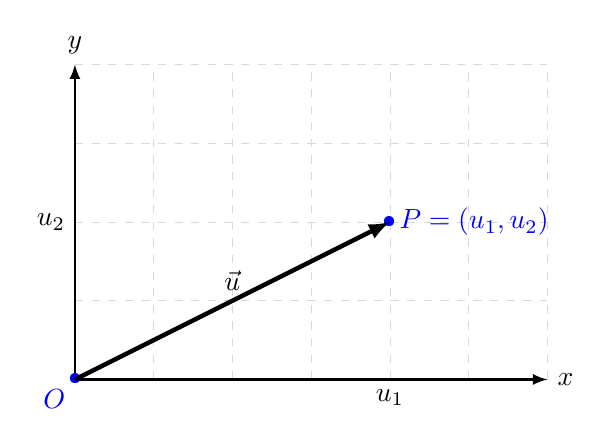
\begin{tikzpicture}[scale=1]
		\tikzset{>=latex}
	\draw[help lines, color=gray!30, dashed] (0,0) grid (6,4);
	\draw[->,thick] (0,0)--(6,0) node[right]{$x$};
	\draw[->,thick] (0,0)--(0,4) node[above]{$y$};
%	\foreach \i in {1,...,7}
%	\node[below,scale=0.7] at (\i,0) {$\i$};
%	\foreach \i in {1,...,4}
%	\node[left,scale=0.7] at (0,\i) {$\i$};


\coordinate (O) at (0,0);
\coordinate (E) at (4,2);
\node[left,scale=1] at (0,2) {$u_2$};
\node[below,scale=1] at (4,0) {$u_1$};

	\node[blue] at (O) {\textbullet};
\node[blue,below left] at (O) {$O$};
	
\node[blue] at (E) {\textbullet};
\node[blue,right] at (E) {$P=(u_1,u_2)$};

\node[above] at (2,1) {$\vec{u}$};

\draw[->,ultra thick] (O) -- (E);
	
	\end{tikzpicture}
\end{center}

Neste caso, escrevemos $\vec{u}=\overrightarrow{OP}$. 

\end{frame}

\subsection*{Norma de um vetor}
\begin{frame}[label=vetores]{Norma de um vetor}

O {\color{blue}comprimento} de vetor $\vec{u}$, também chamado de {\color{blue}norma}, é dado por:

\begin{center}
\begin{minipage}{0.5\textwidth}
\begin{block}{}
\[\|\vec{u}\|=\sqrt{u_1^2+u_2^2}.\]
\end{block}
\end{minipage}
\end{center}


\begin{exe}
Represente no plano o vetor $\vec{u}=(1,1)$ e calcule seu comprimento.
\end{exe}
\end{frame}

\subsection*{Lei do Paralelogramo}

\begin{frame}[label=vetores]{Representação Geométrica da Soma}

Dados dois vetores ${\color{red}\vec{u}=(u_1,u_2)}$ e ${\color{blue}\vec{v}=(v_1,v_2)}$ de $\R^2$  o vetor soma 
\[\vec{u}+\vec{v}=(u_1+v_1,u_2+v_2)\]
é obtido pela chamada {\color{blue}lei do paralelogramo}.

\begin{center}
		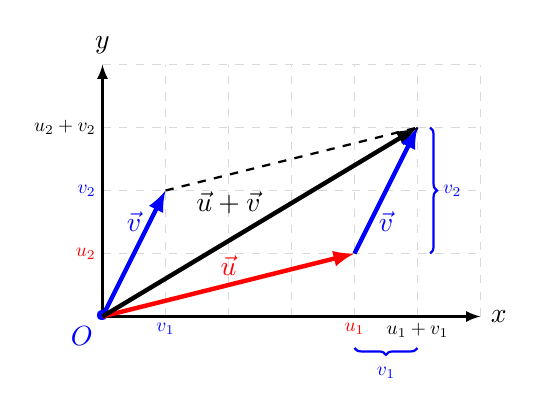
\begin{tikzpicture}[scale=0.8]
		\tikzset{>=latex}
	\draw[help lines, color=gray!30, dashed] (0,0) grid (6,4);
	\draw[->,thick] (0,0)--(6,0) node[right]{$x$};
	\draw[->,thick] (0,0)--(0,4) node[above]{$y$};



\coordinate (O) at (0,0);
\coordinate (A) at (1,2);
\coordinate (B) at (4,1);
\coordinate (C) at (5,3);
\node[red,left,scale=.7] at (0,1) {$u_2$};
\node[red,below,scale=.7] at (4,0) {$u_1$};

\node[blue,left,scale=0.7] at (0,2) {$v_2$};
\node[blue, below,scale=0.7] at (1,0) {$v_1$};

\node[left,scale=.7] at (0,3) {$u_2+v_2$};
\node[below,scale=.7] at (5,0) {$u_1+v_1$};

\node at (2,0.8) {${\color{red}\vec{u}}$};
\node<1> at (0.5,1.5) {${\color{blue}\vec{v}}$};
\node<2> at (4.5,1.5) {${\color{blue}\vec{v}}$};
\node at (2,1.8) {$\vec{u}+\vec{v}$};
\node[blue] at (O) {\textbullet};
\node[blue,below left] at (O) {$O$};

\draw<2>[blue,thick, decorate,decoration = {brace,mirror}] (4,-.5) --  (5,-.5);
\node<2>[blue, below,scale=0.7] at (4.5,-.7) {$v_1$};

\draw<2>[blue,thick, decorate,decoration = {brace,mirror}] (5.2,1) --  (5.2,3);
\node<2>[blue,right,scale=0.7] at (5.3,2) {$v_2$};
	
\draw<1>[->,ultra thick,blue] (O) -- (A);
\draw[->,ultra thick,red] (O) -- (B);
\draw[->,ultra thick] (O) -- (C);

\draw<1>[dashed,thick] (A) -- (C);
\draw<1>[dashed,thick] (B) -- (C);
\draw<2>[->,ultra thick,blue] (B) -- (C);
	
	\end{tikzpicture}
\end{center}



\end{frame}

\subsection*{Coordenadas de um Vetor}

\begin{frame}[label=vetores]

Dizemos que um segmento de reta orientado {\color{red}$\overrightarrow{AB}$} também representa um vetor ${\color{blue}\vec{u}}$ quando os dois têm mesmo {\color{blue}comprimento, direção e sentido}. Neste caso, escrevemos ${\color{blue}\vec{u}}={\color{red}\overrightarrow{AB}}$.



\begin{center}
		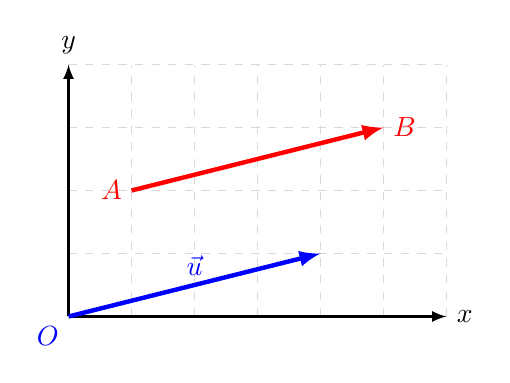
\begin{tikzpicture}[scale=0.8]
		\tikzset{>=latex}
	\draw[help lines, color=gray!30, dashed] (0,0) grid (6,4);
	\draw[->,thick] (0,0)--(6,0) node[right]{$x$};
	\draw[->,thick] (0,0)--(0,4) node[above]{$y$};



\coordinate (O) at (0,0);
\coordinate (A) at (1,2);
\coordinate (B) at (4,1);
\coordinate (C) at (5,3);

\node at (2,0.8) {${\color{blue}\vec{u}}$};
\node[blue,below left] at (O) {$O$};
\node[red,left] at (A) {$A$};
\node[red,right] at (C) {$B$};
	
\draw<1>[->,ultra thick,blue] (O) -- (B);

\draw[->,ultra thick,red] (A) -- (C);
	\end{tikzpicture}
\end{center}

\begin{center}
\begin{minipage}{0.7\textwidth}
\begin{block}{}
Se {\color{red}$A=(a_1,a_2)$} e {\color{red}$B=(b_1,b_2)$} então
\[{\color{red}\overrightarrow{AB}}={\color{blue}\vec{u}=(b_1-a_1,b_2-a_2)}.\]
\end{block}
\end{minipage}
\end{center}

\end{frame}

\begin{frame}[label=vetores]
De uma forma geral temos que 
\begin{center}
\begin{minipage}{0.7\textwidth}
\begin{block}{}
\[\|{\color{red}\overrightarrow{AB}}\|=\sqrt{{\color{blue}(b_1-a_1)^2+(b_2-a_2)^2}}.\]
\end{block}
\end{minipage}
\end{center}


\begin{exe}
Dados $A=(1,1)$, $B=(2,2)$, $C=(-1,0)$ e $D=(0,1)$. Mostre que $\overrightarrow{AB}=\overrightarrow{CD}$ e calcule sua norma.
\end{exe}

\end{frame}




\begin{frame}[label=vetores]


Basta usar a lei do paralelogramo. 

\begin{center}
		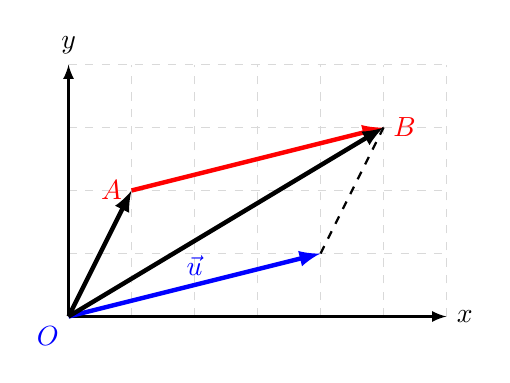
\begin{tikzpicture}[scale=0.8]
		\tikzset{>=latex}
	\draw[help lines, color=gray!30, dashed] (0,0) grid (6,4);
	\draw[->,thick] (0,0)--(6,0) node[right]{$x$};
	\draw[->,thick] (0,0)--(0,4) node[above]{$y$};



\coordinate (O) at (0,0);
\coordinate (A) at (1,2);
\coordinate (B) at (4,1);
\coordinate (C) at (5,3);

\node at (2,0.8) {${\color{blue}\vec{u}}$};
\node[blue,below left] at (O) {$O$};
\node[red,left] at (A) {$A$};
\node[red,right] at (C) {$B$};
	
\draw<1>[->,ultra thick,blue] (O) -- (B);

\draw[->,ultra thick,red] (A) -- (C);
\draw[->,ultra thick] (O) -- (A);
\draw[->,ultra thick] (O) -- (C);
\draw[dashed,thick] (B) -- (C);
	\end{tikzpicture}
\end{center}



Se {\color{blue}$\vec{u}=(x,y)$}, então
\[\overrightarrow{OA}+{\color{blue}\vec{u}}=\overrightarrow{OB}\Rightarrow (a_1+{\color{blue}x},a_2+{\color{blue}y})=(b_1,b_2),\]
donde
\[\begin{cases}
{\color{blue}x}=b_1-a_1\\
{\color{blue}y}=b_2-a_2.
\end{cases}\]

\end{frame}


\begin{frame}[label=vetores]

Em resumo, dados $A=(a_1,a_2)$ e $B=(b_1,b_2)$, escrevemos
\[\overrightarrow{AB}=(b_1-a_1,b_2-a_2).\]

Além disso, se tomarmos vetores $\overrightarrow{AB}$ e $\overrightarrow{BC}$, podemos escrever a soma da seguinte forma:
\[{\color{blue}\overrightarrow{AB}}+{\color{red}\overrightarrow{BC}}=\overrightarrow{AC}.\]

\begin{center}
		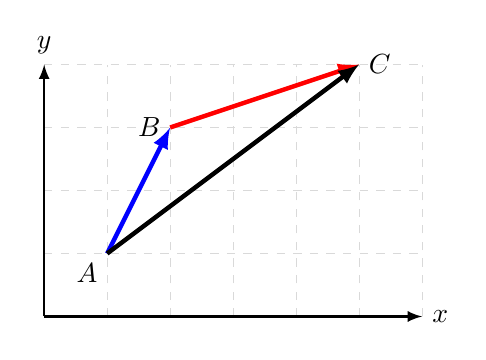
\begin{tikzpicture}[scale=0.8]
		\tikzset{>=latex}
	\draw[help lines, color=gray!30, dashed] (0,0) grid (6,4);
	\draw[->,thick] (0,0)--(6,0) node[right]{$x$};
	\draw[->,thick] (0,0)--(0,4) node[above]{$y$};



\coordinate (O) at (1,1);
\coordinate (A) at (2,3);
\coordinate (B) at (4,1);
\coordinate (C) at (5,4);

\node[below left] at (O) {$A$};
\node[left] at (A) {$B$};
\node[right] at (C) {$C$};
	
\draw<1>[->,ultra thick,blue] (O) -- (A);

\draw[->,ultra thick,red] (A) -- (C);
\draw[->,ultra thick] (O) -- (C);

	\end{tikzpicture}
\end{center}


\end{frame}



\begin{frame}[label=vetores]


\begin{casa}
Localize os pontos $A=(1,1)$, $B=(-3,0)$, $C=(4,1)$, $D=(2,-3)$ e $E=(3,-2)$ no plano cartesiano. Determine as coordenadas dos vetores abaixo e esboce um de seus representantes.
			
\begin{enumerate}
\item $\vt{u}=\vt{AB}+\vt{AC}+\vt{AD}$
				
\item $\vec{v}=2(\vt{BC}-\vt{EC})+3\vt{EA}-2\vt{AD}$
	
\end{enumerate}
\end{casa}

\end{frame}


\begin{frame}[label=vetores]{Representação Geométrica do Produto por Escalar}
Geometricamente, a {\color{blue}multiplicação escalar} estica, contrai ou troca de sentido um vetor.


	\begin{center}
		\begin{tikzpicture}
		\tikzset{>=latex}
%			
	\onslide<2->{\draw<1->[->, thick,blue] (0,0) -- (4,1);}
\onslide<2->{	\node[above ,blue] at (4,1) {$2\vect{u}$};}
\onslide<1->{\draw<1->[->,ultra thick] (0,0) -- (2,.5);
		\node[above ] at (2,0.5) {$\vect{u}$};}

	\onslide<3->{\draw[->, thick,red] (0,0) -- (-4,-1);}
	\onslide<3->{\node[above left ,red] at (-4,-1) {$-2\vect{u}$};}
	\onslide<4->{\draw[->, ultra thick,green] (0,0) -- (1,.25);
	\node[above,green ] at (1,0.25) {$\frac{1}{2}\vect{u}$};	}
		\end{tikzpicture}
	\end{center}

\end{frame}